
\subsection{Regression Results}
\begin{table}[h]
    \centering
    \small
    {
\def\sym#1{\ifmmode^{#1}\else\(^{#1}\)\fi}
\begin{tabular}{l*{4}{c}}
\hline\hline
            &\multicolumn{1}{c}{(1)}&\multicolumn{1}{c}{(2)}&\multicolumn{1}{c}{(3)}&\multicolumn{1}{c}{(4)}\\
            &\multicolumn{1}{c}{Total}&\multicolumn{1}{c}{Between}&\multicolumn{1}{c}{Within}&\multicolumn{1}{c}{Random}\\
\hline
lemp        &       0.496\sym{***}&       0.473\sym{***}&       0.685\sym{***}&       0.598\sym{***}\\
            &     (22.44)         &     (11.15)         &     (23.16)         &     (23.94)         \\
[1em]
ldnpt       &       0.460\sym{***}&       0.481\sym{***}&       0.180\sym{***}&       0.335\sym{***}\\
            &     (31.98)         &     (18.00)         &      (6.74)         &     (17.32)         \\
[1em]
ldrst       &      0.0335\sym{*}  &      0.0315         &      0.0989\sym{***}&      0.0645\sym{***}\\
            &      (2.19)         &      (1.09)         &      (3.63)         &      (3.34)         \\
[1em]
73.yr       &           0         &           0         &           0         &           0         \\
            &         (.)         &         (.)         &         (.)         &         (.)         \\
[1em]
78.yr       &      0.0137         &           0         &      0.0484\sym{**} &      0.0266         \\
            &      (0.42)         &         (.)         &      (2.93)         &      (1.59)         \\
[1em]
83.yr       &      -0.125\sym{***}&           0         &     -0.0107         &     -0.0762\sym{***}\\
            &     (-3.75)         &         (.)         &     (-0.53)         &     (-4.10)         \\
[1em]
88.yr       &       0.163\sym{***}&           0         &       0.244\sym{***}&       0.196\sym{***}\\
            &      (4.87)         &         (.)         &     (11.18)         &     (10.22)         \\
[1em]
d357\_73     &      -3.235\sym{***}&      -5.688\sym{***}&      -3.421\sym{***}&      -3.295\sym{***}\\
            &    (-30.20)         &    (-14.44)         &    (-44.68)         &    (-29.94)         \\
[1em]
d357\_78     &      -2.064\sym{***}&           0         &      -2.286\sym{***}&      -2.143\sym{***}\\
            &    (-19.22)         &         (.)         &    (-30.44)         &    (-19.37)         \\
[1em]
d357\_83     &      -0.689\sym{***}&           0         &      -0.944\sym{***}&      -0.791\sym{***}\\
            &     (-6.38)         &         (.)         &    (-12.73)         &     (-7.09)         \\
[1em]
d357\_88     &       0.240\sym{*}  &           0         &           0         &       0.144         \\
            &      (2.22)         &         (.)         &         (.)         &      (1.29)         \\
[1em]
\_cons      &       2.887\sym{***}&       2.838\sym{***}&       3.717\sym{***}&       3.208\sym{***}\\
            &     (52.89)         &     (27.84)         &     (32.26)         &     (45.04)         \\
\hline
\(N\)       &         856         &         856         &         856         &         856         \\
\hline\hline
\multicolumn{5}{l}{\footnotesize \textit{t} statistics in parentheses}\\
\multicolumn{5}{l}{\footnotesize \sym{*} \(p<0.05\), \sym{**} \(p<0.01\), \sym{***} \(p<0.001\)}\\
\end{tabular}
}

    \caption{Regression Results}
    \label{tab:my_label}
\end{table}

In model Total, since dummy variables for year are linearly correlated, one of them (\textit{77.yr}) does not have an estimation. Moreover, in model Between, since we first take average within each group, coefficient of year dummies do not make a sense (Because there is no variation between groups). Also, since industry during time does not change, just one of the 4 d357 time dummies, can be estimated. 
Also, we can see that the estimates are different, in particular, the within-estimate of labor and R&D are higher than the other estimates. 

\subsection{Hausman Test}

The Hausman test is 59.15 ($\chi^2$ with 9 degrees of freedom) and is rejected with p-value $<$ 0.001. Therefore, the random effects specification is not valid.

\begin{figure}[h]
    \centering
    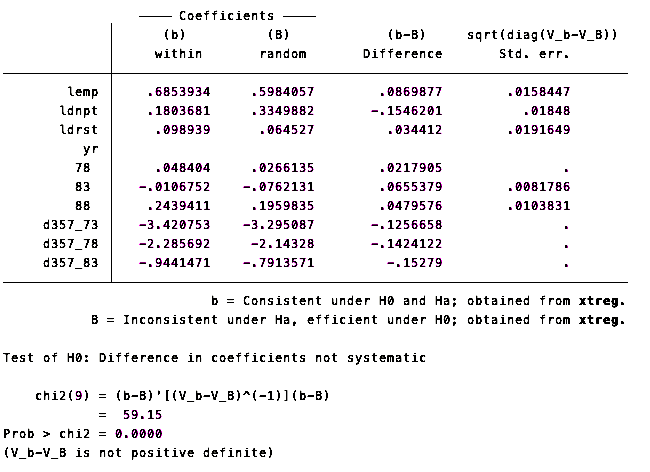
\includegraphics[scale=0.5]{HW1/LATEX/Attachments/Q2_2.png}
    \caption{Hausman Test}
    \label{fig:my_label}
\end{figure}

\subsection{What we learn?}

This suggests that the random effects specification is not valid, and there are systematic differences across firms that are related to input choices. In particular, the underestimation of the labor coefficient might imply that some companies have more efficient managers, so fewer workers are required — and knowing this, a company hires less. The underestimation of the R&D capital can similarly reflect that some companies are more efficient and have a higher return on R&D, therefore, they do not invest as much as other firms.